\input templates/header
\title[DS - Complex Network]{\textbf{Distributed Algorithms}\\Complex Networks}

\graphicspath{{figs/08/}}

\begin{document}

\newcommand{\Path}{\ell}
\newcommand{\Diam}{\mathit{diam}}

\FrameTitle{
	\begin{tabular}{P{2.8cm} P{8cm}}
		Acknowledgments: & 
		Mark Jelasity, Sebastian Ahnert, Lada Adamic, Albert Diaz Guilera\\
	\end{tabular}
}

\FrameContent

%%%%%%%%%%%%%%%%%%%%%%%%%%%%%%%%%%%%%%%%%%%%%%%%%%%%%%%%%%%%%%%%%%%%%%%%

\section{Introduction}

\begin{frame}{Introduction}

\begin{block}{What these structures have in common?}

\begin{columns}
\begin{column}{0.5\textwidth}
\BI
\item World Wide Web
\item Internet
\item Movie actor collaborations
\item Science collaborations
\item Citations of papers
\item Sexual relationships
\EI
\end{column}
\begin{column}{0.5\textwidth}
\BI
\item Food webs
\item Facebook \& Linkedin
\item Co-occurrence of words
\item Your brain
\item The power network of USA
\item Protein folding
\EI
\end{column}
\end{columns}
\end{block}

\pause
\bigskip
\BI
\item They can be described as graphs
\pause
\item They all show similar features!
\EI

\end{frame}


\begin{frame}{Brief historical overview:}
	
\BIL
\item 1736:		 	Graph theory (Euler)
\item 1937:			Journal Sociometry founded
\item 1959:			Random graphs (Erdős-Rényi)
\item 1967:			Small-world (Milgram)
\item 1990s:		“Complex networks” 	 
\EIL

\end{frame}


\begin{frame}{Complex network research}

\BIL
\item Rapidly increasing interest over the last decade, since much more network data available now
\item Multidisciplinary research 
  \BI
  \item Physics
  \item Biology
  \item Sociology
  \item Mathematics
  \item Epidemiology
  \item \ldots
  \EI
\item Strong implications for Computer Science
\BI
\item Robustness of networks
\item Efficiency: function of networks depends on their structure
\item Design and engineering
\EI
\EIL
\end{frame}

\begin{frame}{Complex network research}

\begin{columns}
\begin{column}{0.4\textwidth}
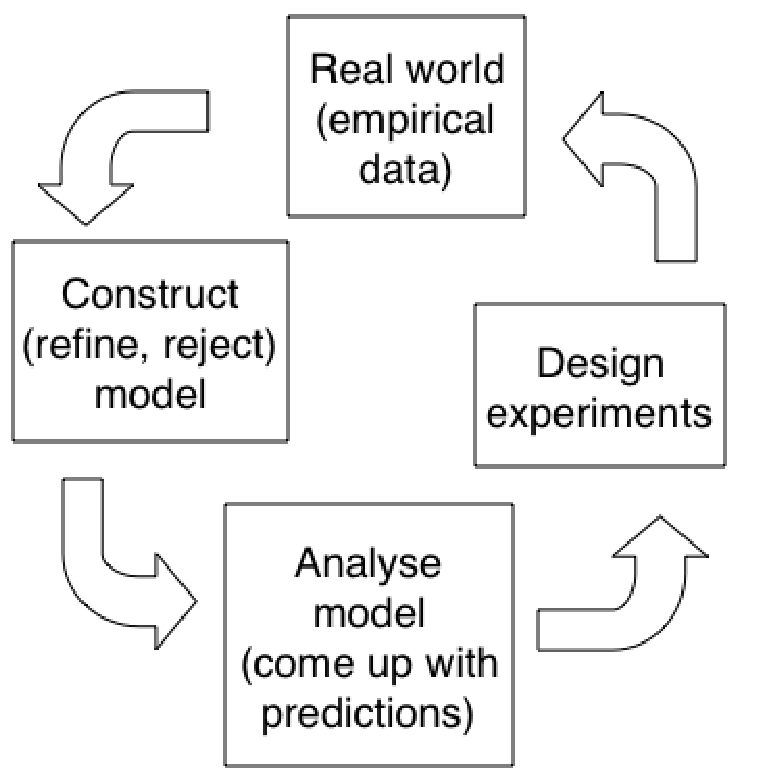
\includegraphics[width=\textwidth]{experimental}
\end{column}
\begin{column}{0.6\textwidth}
\BIL
\item Complex networks is a branch of physics
\item Empirical science: loop of modeling and observation
\item Models are models
\BI
\item Explain some aspects
\item Don't explain other aspects
\EI
\item Has a lot to do with condensed matter physics
\EIL
\end{column}
\end{columns}


\end{frame}

\section{Topological properties}

\subsection{Degree statistics}

\begin{frame}{Degree statistics (1)}

\begin{definition}[Degree]
\BI
\item The \alert{degree} $k_i$ of node $i$ is the number of edges the node has to other nodes
\item In this lecture, we will only consider undirected graphs
\item Called \alert{local centrality} in social network analysis
\item Measures how important is a node with respect to its neighbors
\EI
\end{definition}	

\begin{figure}
	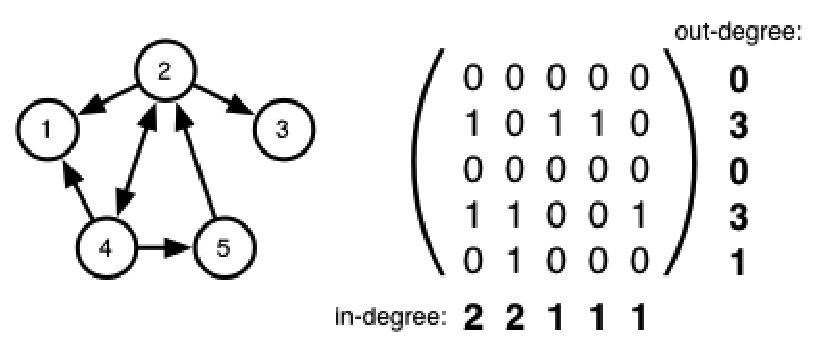
\includegraphics[width=0.75\textwidth]{degree}
\end{figure}


\end{frame}

\begin{frame}{Degree statistics (2)}

\begin{definition}[Degree distribution]
\BI
\item The average degree of a graph $G=(V,E)$ is $\langle k \rangle = \frac{|E|}{|V|}$ 
\item $P(k)$ is the probability that a random node has degree $k$
\item The probability distribution gives an idea of the spread in the number of links the nodes have
\EI
\end{definition}

\begin{figure}
	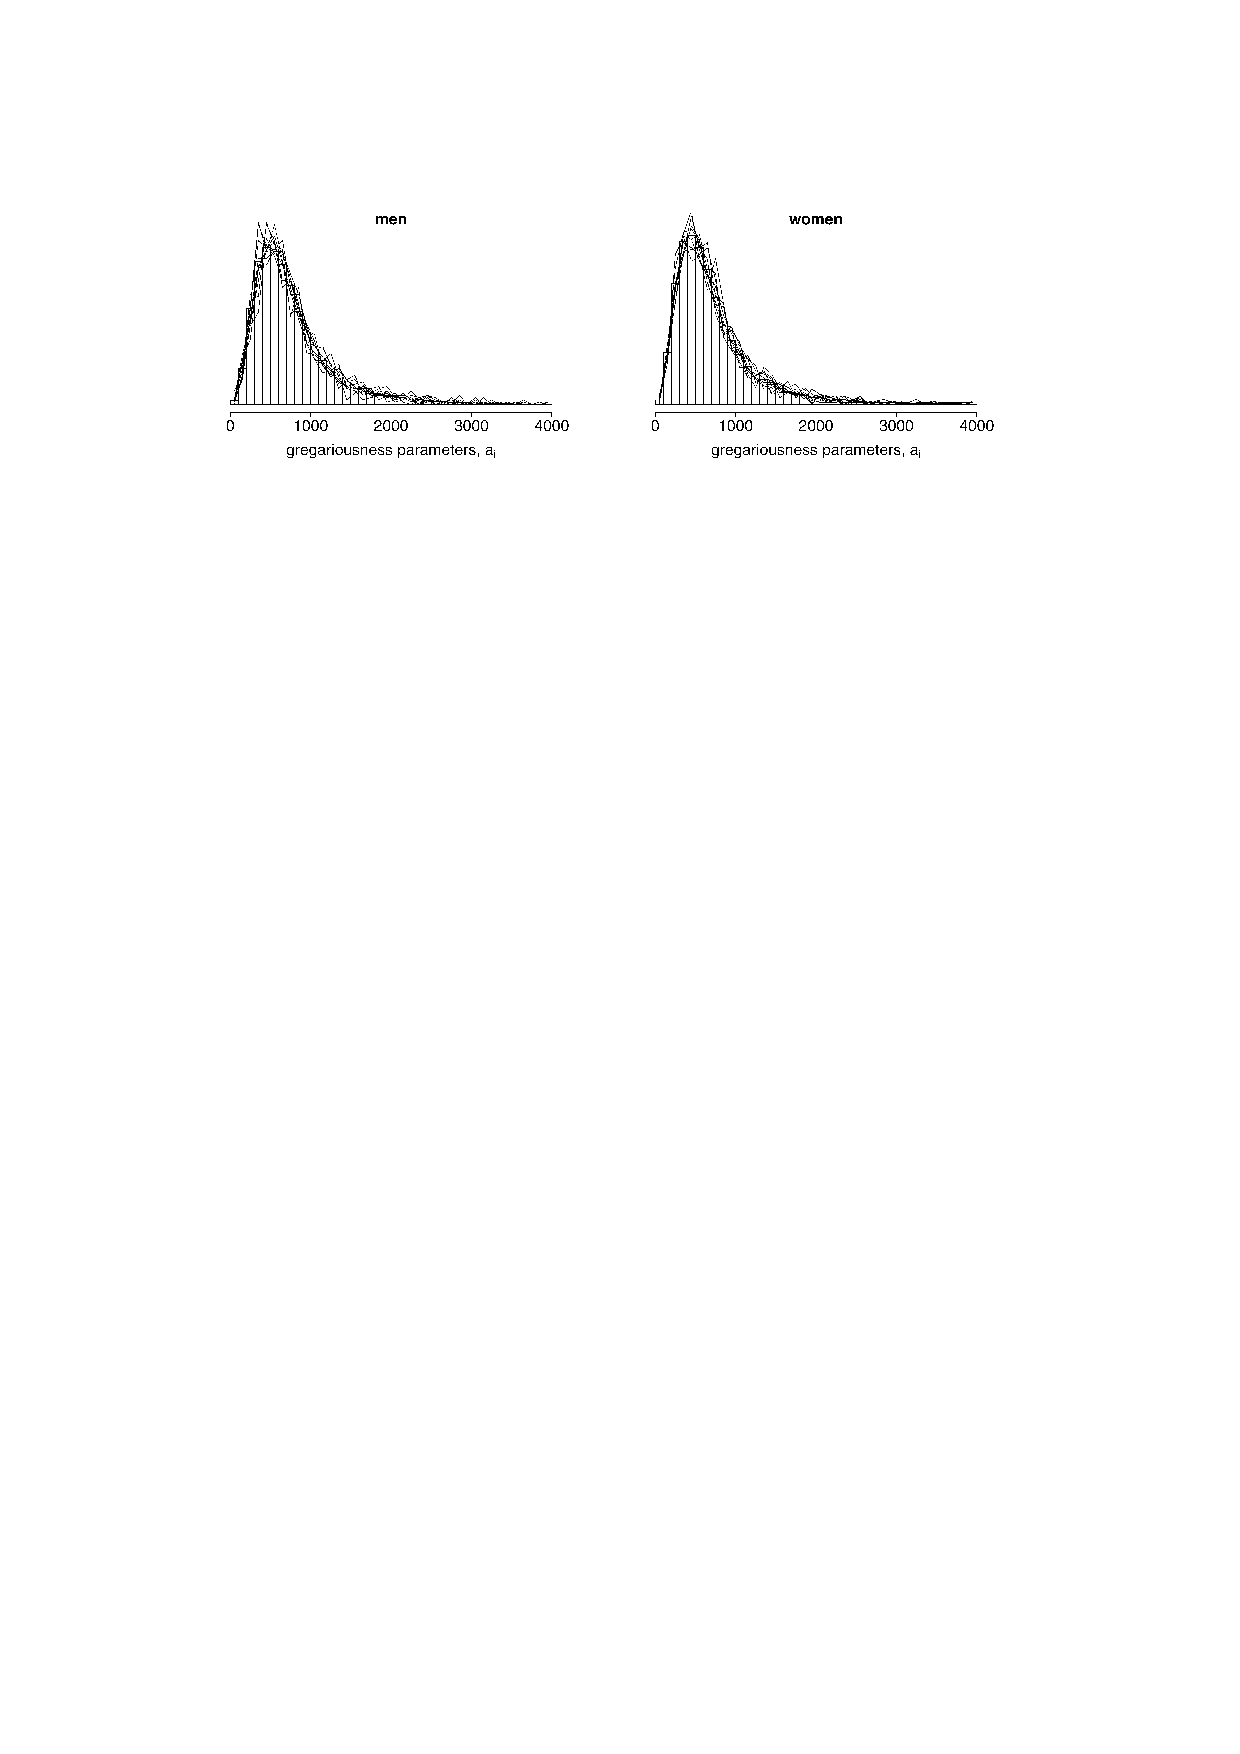
\includegraphics[width=0.8\textwidth]{degreedist}
\end{figure}
	
\note{
Tian ZHENG, Matthew J. SALGANIK, and Andrew GELMAN. How Many People Do You Know in Prison?: Using
Overdispersion in Count Data to Estimate Social Structure in Networks. In Journal of the American Statistical Association, 2006
}	
	
\end{frame}

\subsection{Distance statistics}

\begin{frame}{Distance statistics (1)}

\begin{definition}[Path length]
The \alert{path length} $d(i,j)$, or \alert{goedesic distance}, between two nodes $i$ and $j$ is the length
of the shortest path connecting them. 
\end{definition}

\begin{figure}
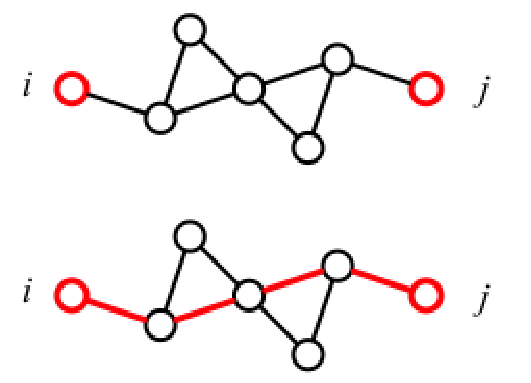
\includegraphics[width=0.6\textwidth]{distance}
\end{figure}

\end{frame}

\begin{frame}{Distance statistics (2)}
	
\begin{definition}[Average path length]
The \alert{average path length} of a connected graph $G=(V,E)$ is defined as:
\[
  \Path(G) = \frac{1}{|V|(|V|-1)} \sum_{i,j \in V, i \neq j} d(i,j)
\]
\end{definition}

\begin{figure}
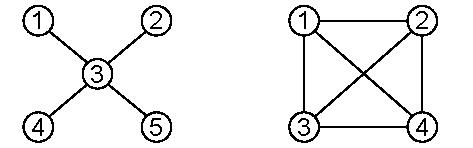
\includegraphics[width=0.6\textwidth]{diameter}
\caption{(a) $\Path(G) = (4 \cdot ((2+2+2+1)/8) + 1)/5=1.6$. (b) $\Path(G) = 1$}
\end{figure}

\end{frame}


\begin{frame}{Distance statistics (3)}

\begin{definition}[Diameter]
The \alert{diameter} is the maximal shortest path between any two vertices:
\[
  \Diam(G) = \max \{ d(i,j) : i,j \in V \}
\]
\end{definition}

\begin{figure}
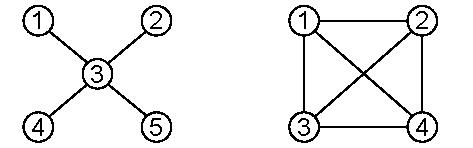
\includegraphics[width=0.6\textwidth]{diameter}
\caption{(a) $\Diam(G) = 2$. (b) $\Diam(G) = 1$}
\end{figure}

\end{frame}

\subsection{Clustering coefficient}

\begin{frame}{Clustering coefficient (1)}

\begin{definition}[Induced graphs]
The subgraph $G_i=(V_i, E_i)$ \alert{induced} by node $i$ over a graph $G=(V,E)$ 
  is given by the neighbors of $i$ and the edges linking them:
  \begin{align*}
	 V_i &= \{ j : j \in V \wedge (i,j) \in E \} \\
	 E_i &= \{ (i,j) : i,j \in V_i \wedge (i,j) \in E \} 
  \end{align*}
\end{definition}

\bigskip
\begin{overprint}
\onslide<1|handout:0>
\begin{figure}
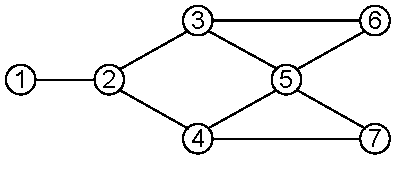
\includegraphics[width=0.7\textwidth]{induced1}
\end{figure}
\onslide<2|handout:1>
\begin{figure}
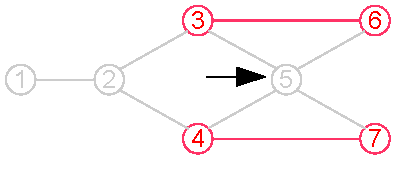
\includegraphics[width=0.7\textwidth]{induced2}
\end{figure}
\end{overprint}
\end{frame}

\begin{frame}{Clustering coefficient (2)}

\begin{definition}[Local clustering coefficient]
The \alert{local clustering coefficient} of node $i$ in graph $G$ is the
  ratio between the size of $|E_i|$ and the number of all potential edges
  that link two nodes in $V_i$:
  \[
     CC(G,i) = \frac{|E_i|}{|V_i|(|V_i|-1)/2} = \frac{2|E_i|}{|V_i|(|V_i|-1)}
  \]
\end{definition}

\begin{figure}
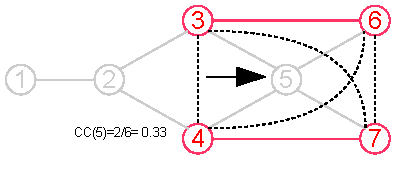
\includegraphics[width=0.7\textwidth]{induced3}
\end{figure}

\end{frame}

\begin{frame}{Clustering coefficient (3)}

\begin{definition}[Clustering coefficient]

The \alert{clustering coefficient} of graph $G$ is the average over the local 
  clustering coefficient of all nodes in the graph
  \[
     CC(G) = \frac{1}{N} \sum_{i \in V} CC(G,i)
  \]
\end{definition}

\begin{columns}
	\begin{column}{0.35\textwidth}
		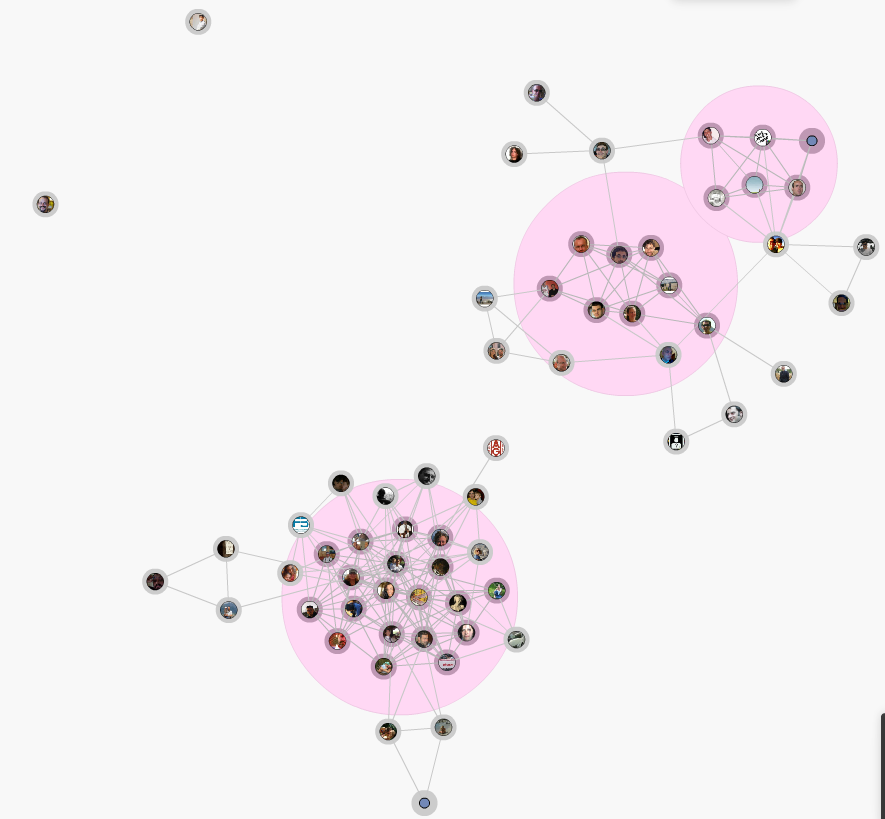
\includegraphics[width=\textwidth]{facebook}
	\end{column}
	\begin{column}{0.65\textwidth}
		\BI
		\item Facebook clustering coefficient 0.16
		\EI
	\end{column}
\end{columns}
\end{frame}

\subsection{Milgram Experiment}

\begin{frame}{The Milgram Small-World Experiment}

Milgram's experiment (1967):

Given a target individual and a particular property, pass the message to a 
person you correspond with who is “closest” to the target.

\begin{figure}
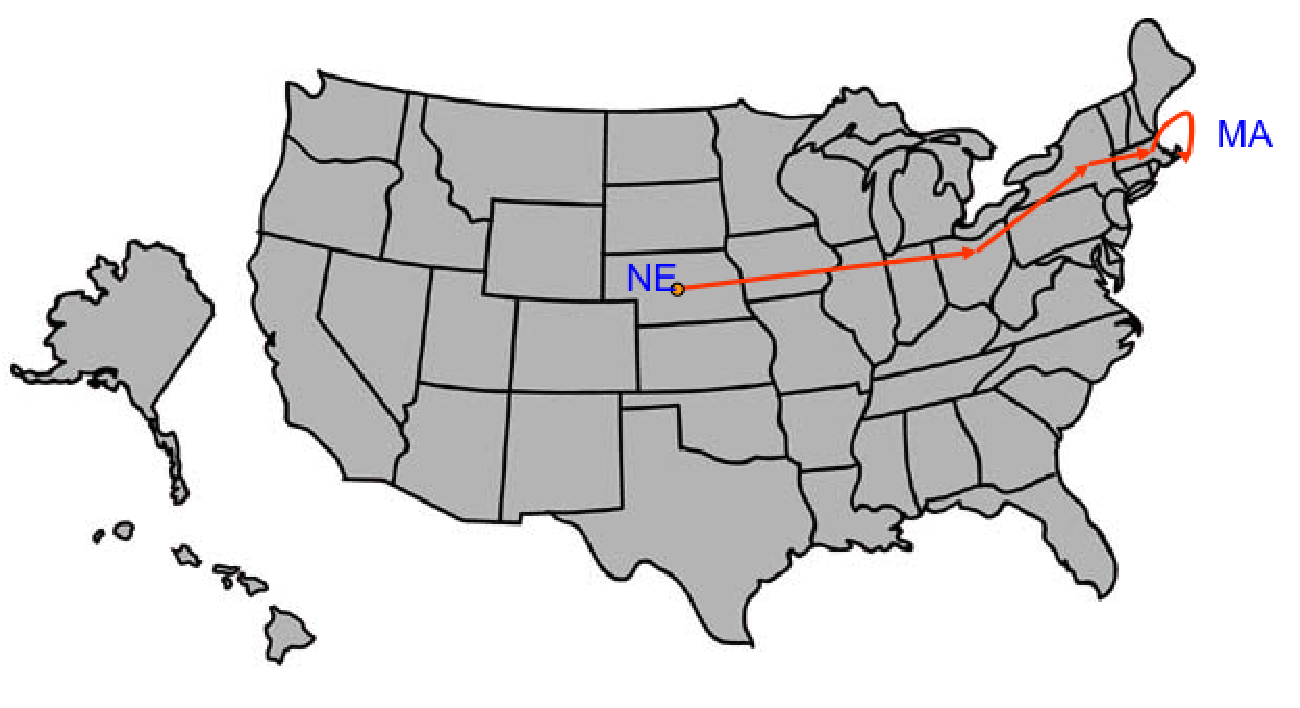
\includegraphics[width=0.8\textwidth]{milgram}
\end{figure}
	
\end{frame}

\begin{frame}{The Milgram Small-World Experiment}
	
\structure{Some facts}:

\BI
\item Target person worked in Boston as a stockbroker.
\item 296 senders from Boston and Omaha.
\item 20\% of senders reached target.
\item Average path length = 6.5.
\EI

\bigskip
\structure{“Six degrees of separation”}:

\BI
\item It's a small world after all!
\item Kevin-Bacon game
\item Erd\"os number
\EI

\end{frame}

\begin{frame}{Six Degrees and Popular Culture}

\begin{columns}
\begin{column}{0.65\textwidth}
\begin{block}{“Everything is Different”\\ Frigyes Karinthy, 1929}
\begin{quote}
{\footnotesize
A fascinating game grew out of this discussion. One of us suggested performing
the following experiment to prove that the population of the Earth is closer
together now than they have ever been before. We should select any person from
the 1.5 billion inhabitants of the Earth—anyone, anywhere at all. He bet us
that, using no more than five individuals, one of whom is a personal
acquaintance, he could contact the selected individual using nothing except
the network of personal acquaintances.}
\end{quote}
\end{block}
\end{column}
\begin{column}{0.35\textwidth}
	
\includegraphics[width=\textwidth]{sixdegrees}
\end{column}
\end{columns}


\note{
\BI
\item Frigyes Karinthy is an Hungarian author.
\item The original ideas come out from Guglielmo Marconi's Nobel lecture - but
 I was not able to find such link in the speech
\item Six Degrees of Separation is a 1993 film drama featuring Will Smith, Donald Sutherland and Stockard Channing
\item Will Smith and Charlie Chaplin have a distance of $3$, through Jack Lemmon and Hank Mann
\EI
}

\end{frame}


\begin{frame}[label=statistics]{Statistics over real networks}
	
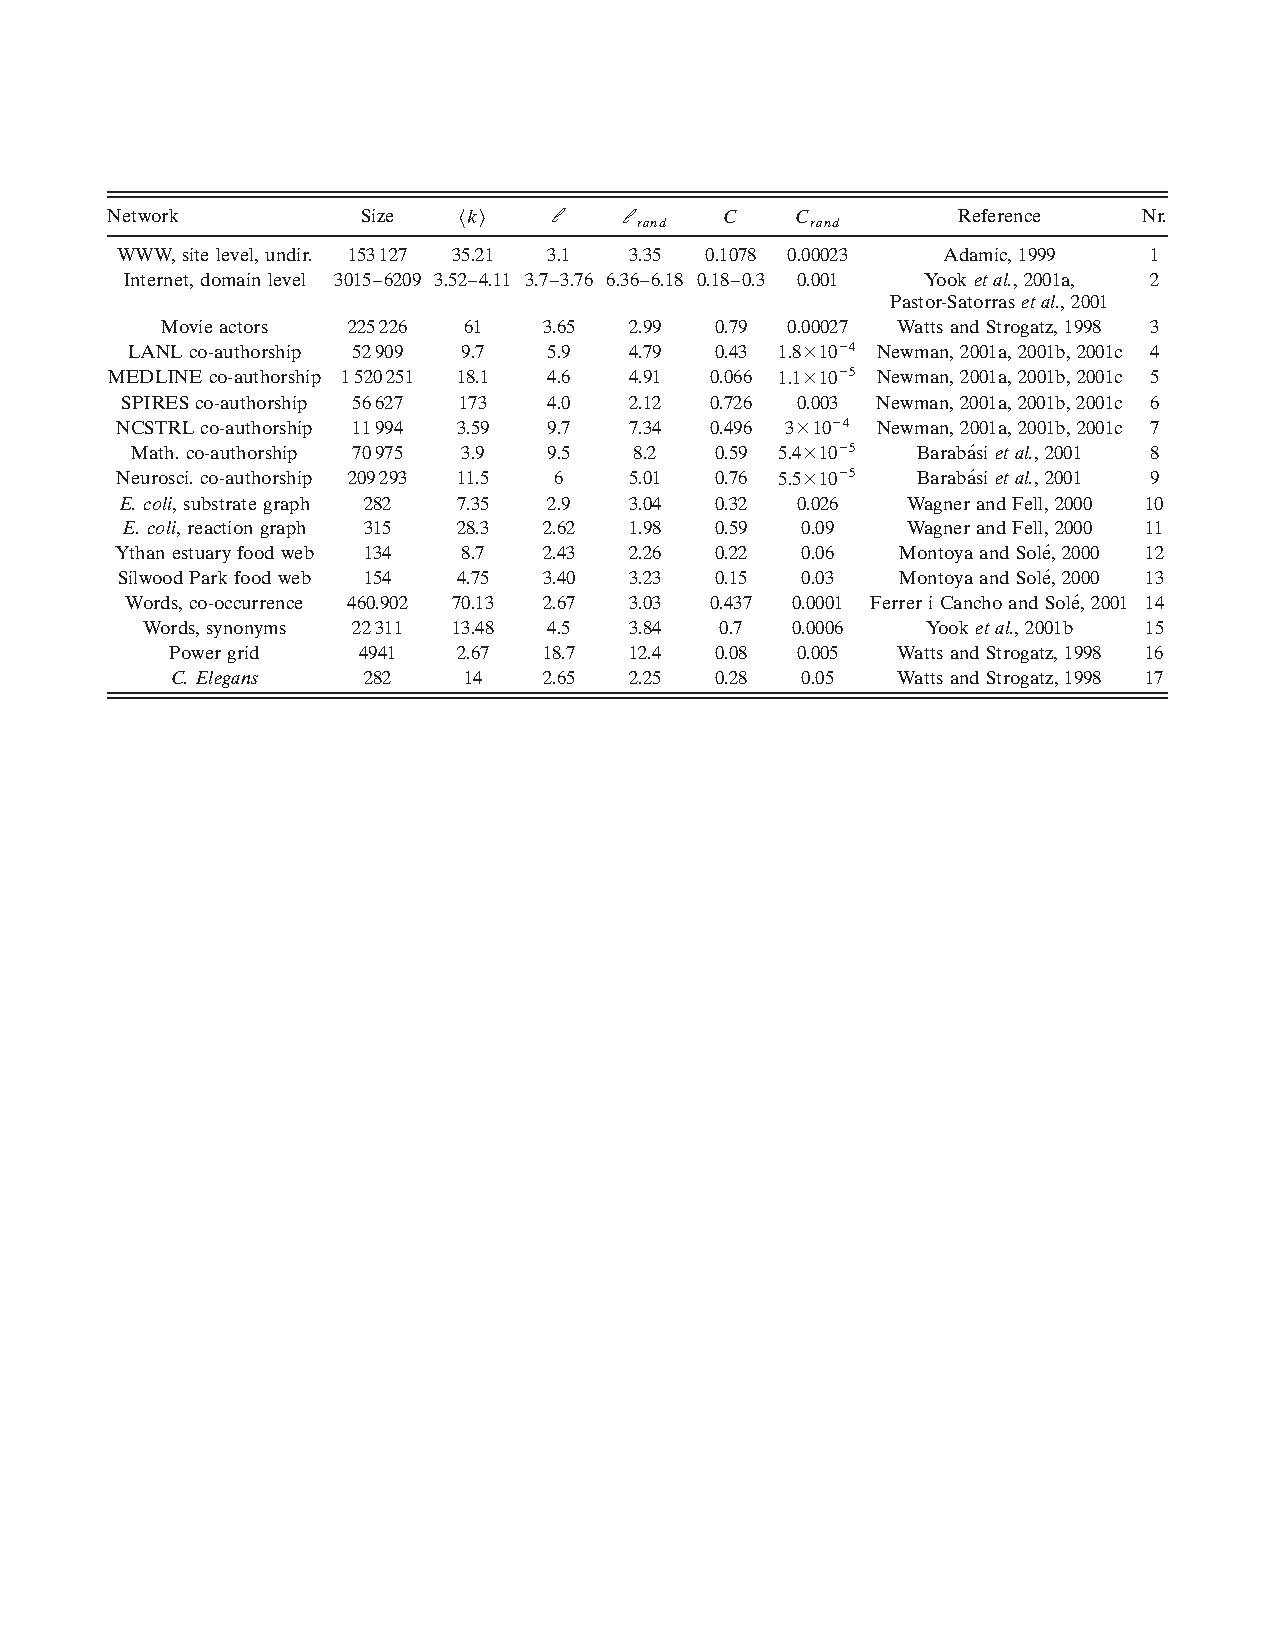
\includegraphics[width=\textwidth]{statistics}
\end{frame}


\section{Graph modeling}

\subsection{Random graphs}

\begin{frame}{Erd\"{o}s-R\'{e}nyi Random (E-R) Networks}

\begin{definition}[Random Graph]
Given a network of $N$ nodes, connect each pair $(p_i,p_j)$ of nodes
with probability $p$
\end{definition}

\bigskip
Two different realizations for $N = 5$ and $p = 0.5$

\begin{figure}
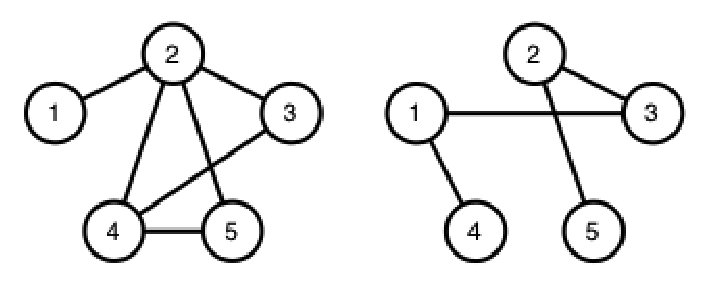
\includegraphics[width=0.5\textwidth]{random}
\end{figure}

\end{frame}

\begin{frame}{Some properties of E-R networks}

\structure{Given an E-R graph with $N$ nodes and probability $p$}:

\BIL
\item Expected number of edges: $|E| = pN(N-1)/2$	
\item Expected average degree: $\langle k \rangle = 2|E|/N = p(N-1) \approx pN$
\item Degree distribution: $P(k) = \binom{N-1}{k} p^k(1-p)^{N-1-k}$ (binomial)
\item In the limit of large $N$, $\Diam(G) = \frac{\log N}{\log \langle k \rangle}$
\item Average path length is bounded by diameter
\item Clustering coefficient: $CC(G) = p$
\EI

\note{
\begin{minipage}{\textwidth}	
\BI
\item This probability represents the number of ways in which $k$ edges can be
drawn from a certain node: the probability of $k$ edges is $p^k$, the
probability of the absence of additional edges is $(1-p)^{N-1-k}$k, and there
are $\binom{N-1}{k}$, equivalent ways of selecting those $k$ edges.
\item Random graphs tend to have small diameters, provided $p$ is not too
small. The reason for this is that a random graph is likely to be spreading:
with large probability the number of nodes at a distance $l$ from a given node
is not much smaller than $\langle k \rangle^l$. Equating $\langle k \rangle^l$
with $N$ we find that the diameter is proportional to $l = \log N / \log k$.
\item If we consider a node in a random graph and its nearest neighbors, the
probability that two of these neighbors are connected is equal to the
probability that two randomly selected nodes are connected.
\EI
\end{minipage}
}

\end{frame}

\begin{frame}{Random networks vs real ones}
\begin{block}{Question}
Are random networks a good model for real networks?
\end{block}	
\end{frame}

\againframe{statistics}

\subsection{Small-world networks}

\begin{frame}{Small-World Networks}

\begin{block}{Answer -- No!}
\BI
\item Average path length of real networks is similar to the one of random networks...
\item ...but their clustering coefficient is many orders of magnitude larger
\EI
\end{block}

\bigskip
\begin{block}{Problem -- Modeling \alert{small-world} networks}
How we can build a network with \alert{small degree}, \alert{small
average path length} and \alert{large clustering coefficient}?
\end{block}

\end{frame}

\begin{frame}{Small-World Networks}

\begin{block}{Watts-Strogatz Model}
Watts and Strogatz (1998) observed that by taking a locally connected 
network and randomly rewiring a small number of edges, the average distance 
between two nodes falls drastically
\end{block}

\begin{figure}
	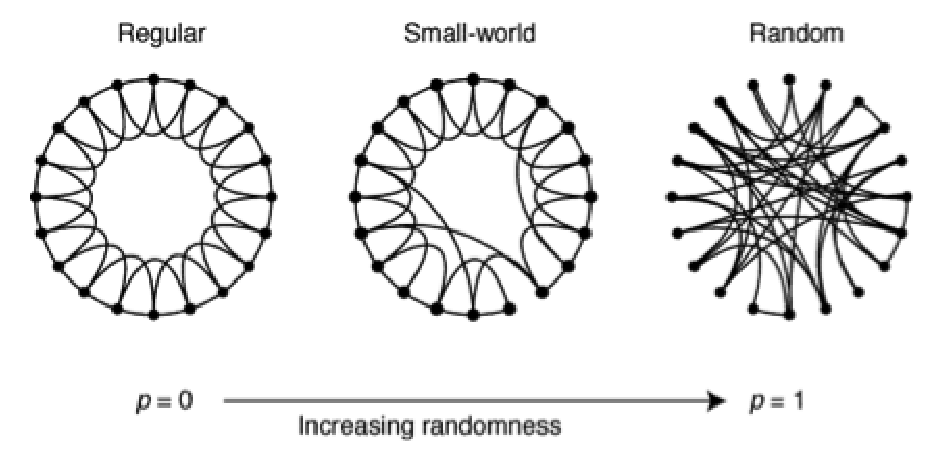
\includegraphics[width=0.7\textwidth]{watts}
\end{figure}

\end{frame}

\begin{frame}{Formal definition}
	
\begin{definition}[Watts-Strogatz Model]
\begin{enumerate}
\item Construct a regular ring lattice, a graph with $N$ nodes each connected to $k$ neighbors, $k/2$ on each side
  \BI
  \item Label nodes $0, 1, \ldots, N-1$
  \item Add an edge $(i,j)$ if and only if $0 < |i-j| \bmod N \leq k/2$
  \EI
\item For every node $i \in [0, N-1]$, take each each every edge $(i,j)$ with $i<j$ and rewire it with probability $p$
  \BI
  \item Replace $(i,j)$ with $(i,k)$ such that $i \neq k$ and $(i,k) \notin E$ 
  \EI
\end{enumerate}
\end{definition}


\end{frame}

\begin{frame}{The small-world region}

\begin{figure}
	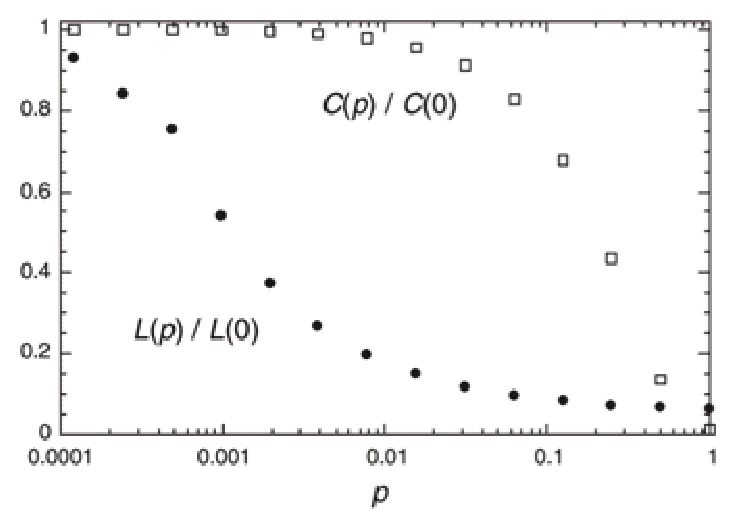
\includegraphics[width=0.8\textwidth]{watts-sim}
\end{figure}
	
\end{frame}

\begin{frame}{Looking back at degree distribution}

\begin{block}{Question}
Are Watts-Strogatz networks a good model for real networks?
\end{block}

\begin{overprint}
\onslide<1|handout:1>

\begin{figure}
	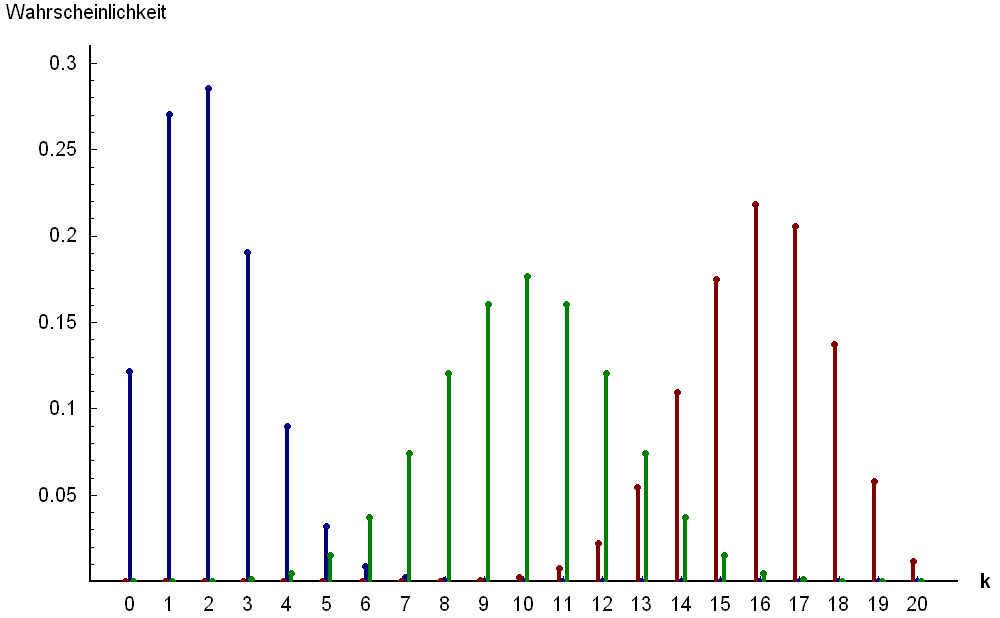
\includegraphics[width=0.6\textwidth]{binomial}
	\caption{Binomial distribution for $n = 20$
$p = 0.1$ (blue), $p = 0.5$ (green) and $p = 0.8$ (red).
{\scriptsize \url{http://en.wikipedia.org/wiki/File:Binomial_Distribution.PNG}}
}
\end{figure}

\onslide<2|handout:2>

\begin{figure}
	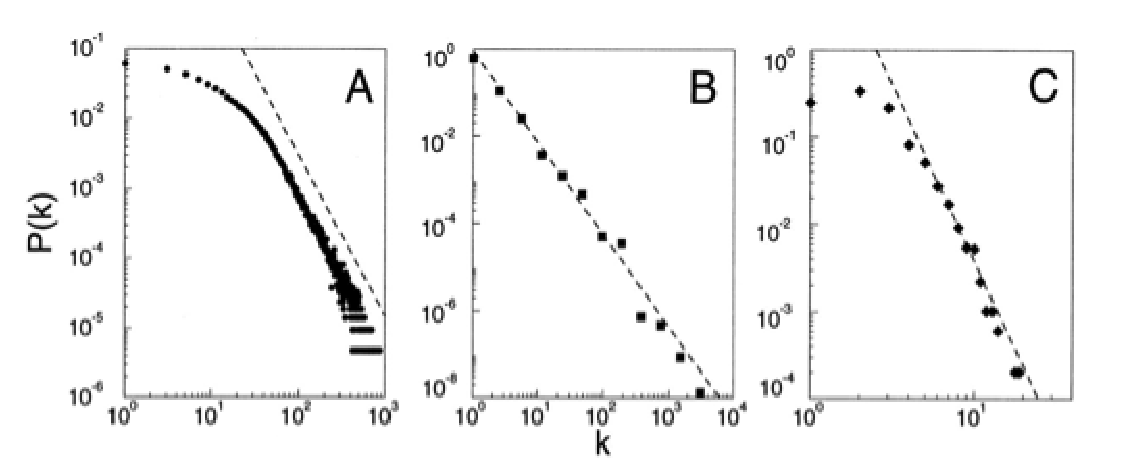
\includegraphics[width=0.9\textwidth]{threeex}
	\caption{Real network degree distributions: from left to right, Actors, WWW, Power grid}
\end{figure}
	
\end{overprint}
	
\end{frame}

\subsection{Scale-Free Networks}

\begin{frame}{Scale-Free Networks}
\BI
\item Many nodes have few connections and a few nodes have many connections
\item This observation holds on the local and global scale of the network
\item In other words, \alert{there is no inherent scale}
\EI

\begin{definition}[Power-law degree distribution]
Formally this translates into a power-law degree distribution: 
\[
  P(k) \propto k^{-\lambda}
\]
\end{definition}

\end{frame}

\begin{frame}{Statistics over real networks}

\begin{columns}
\begin{column}{0.5\textwidth}
\begin{figure}
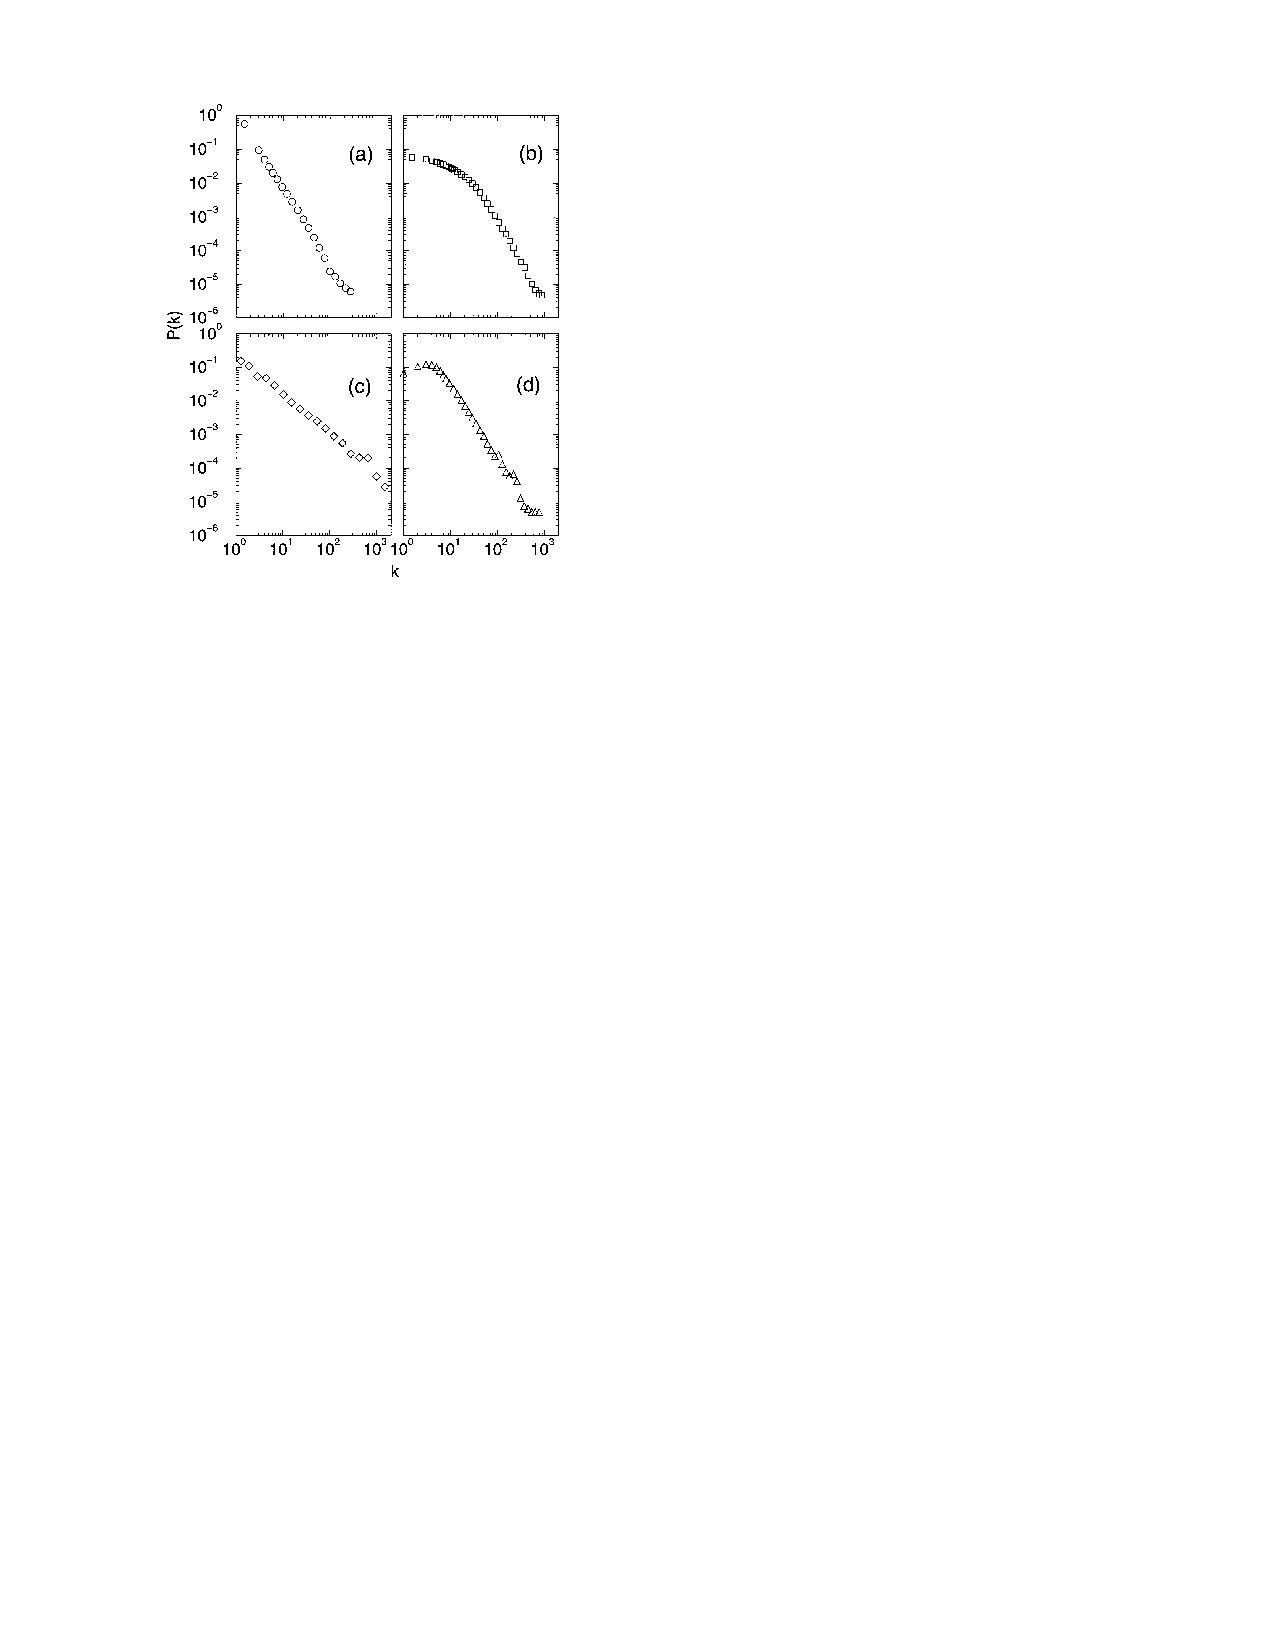
\includegraphics[width=\textwidth]{scalefree}
\end{figure}
\end{column}
\begin{column}{0.5\textwidth}
\BI
\item[(a)] Internet at the router level
\item[(b)] movie actor collaboration network
\item[(c)] co-authorship network of high-energy physicists
\item[(d)] co-authorship network of neuroscientists
\EI
\end{column}
\end{columns}

\end{frame}

\begin{frame}{Statistics over real networks}
	
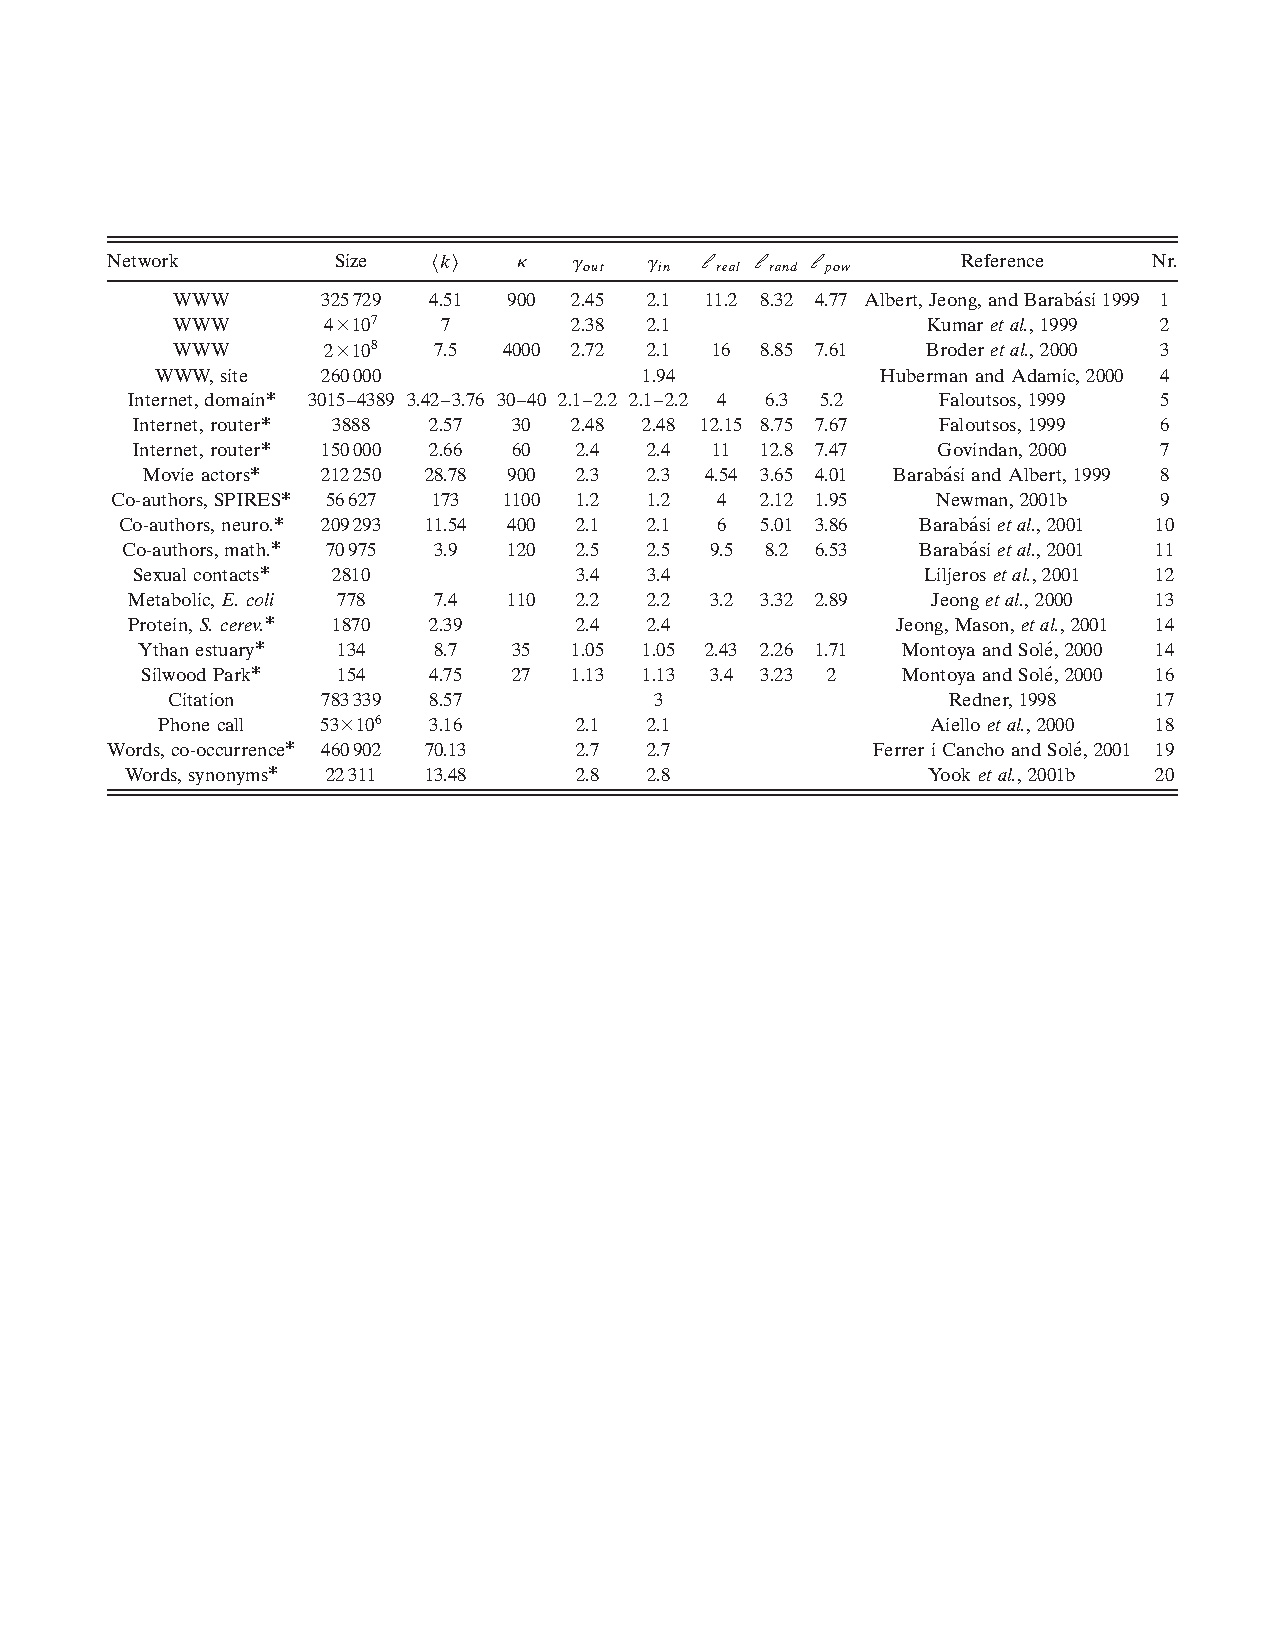
\includegraphics[width=\textwidth]{statistics2}

\end{frame}

\begin{frame}{Barab\'{a}si-Albert Model}

\begin{definition}[Preferential attachment]
\BI
\item Start with a small clique of size $m_0 \geq 3$
\item Repeat adding a new node with $m \leq m_0$ edges
\item New node is connected with node $i$ with a probability proportional to the
number of links that $i$ already has. Formally,
\[
  P(i) = \frac{k_i}{\sum_j k_j}
\]
\EI
\end{definition}

\end{frame}

\begin{frame}{Mathematical properties}

\BI
\item $m_0+t$ nodes, $mt$ edges
\item $P(k) \propto k^{-3}$
\item $\ell(G) = \frac{\log N}{\log \log N}$\\
  (somewhat smaller than random)
\item $CC(G) \approx N^{-0.75}$
\EI

\begin{block}{Summary}
\BI
\item Models degree distribution
\item But doesn’t model clustering
\EI
\end{block}

\end{frame}

\section{Other topological properties}

\begin{frame}{Assortativity}

\BI
\item \alert{Assortativity} describes the correlation between the degree of a node and the degree of its neighbors. 
\item Networks in which highly connected nodes are linked to other nodes with a high degree are termed \alert{assortative}. Such networks include social networks
\item Networks in which highly connected nodes are only linked to nodes with a low degree are termed \alert{disassortative}. Such networks include the World Wide Web and biological networks.
\EI

\end{frame}

\begin{frame}{Robustness}

\begin{columns}
\begin{column}{0.5\textwidth}
\BIL
\item We need to understand how vulnerable existing systems are
\item We need to design self-healing and self-protecting systems
\item Node removal models:
	\BI 
	\item \alert{Random}: a random node is removed along with all the links
	\item \alert{Preferential}: the most connected (highest degree) nodes are removed
	\EI
\EIL
\end{column}
\begin{column}{0.5\textwidth}

\begin{figure}
	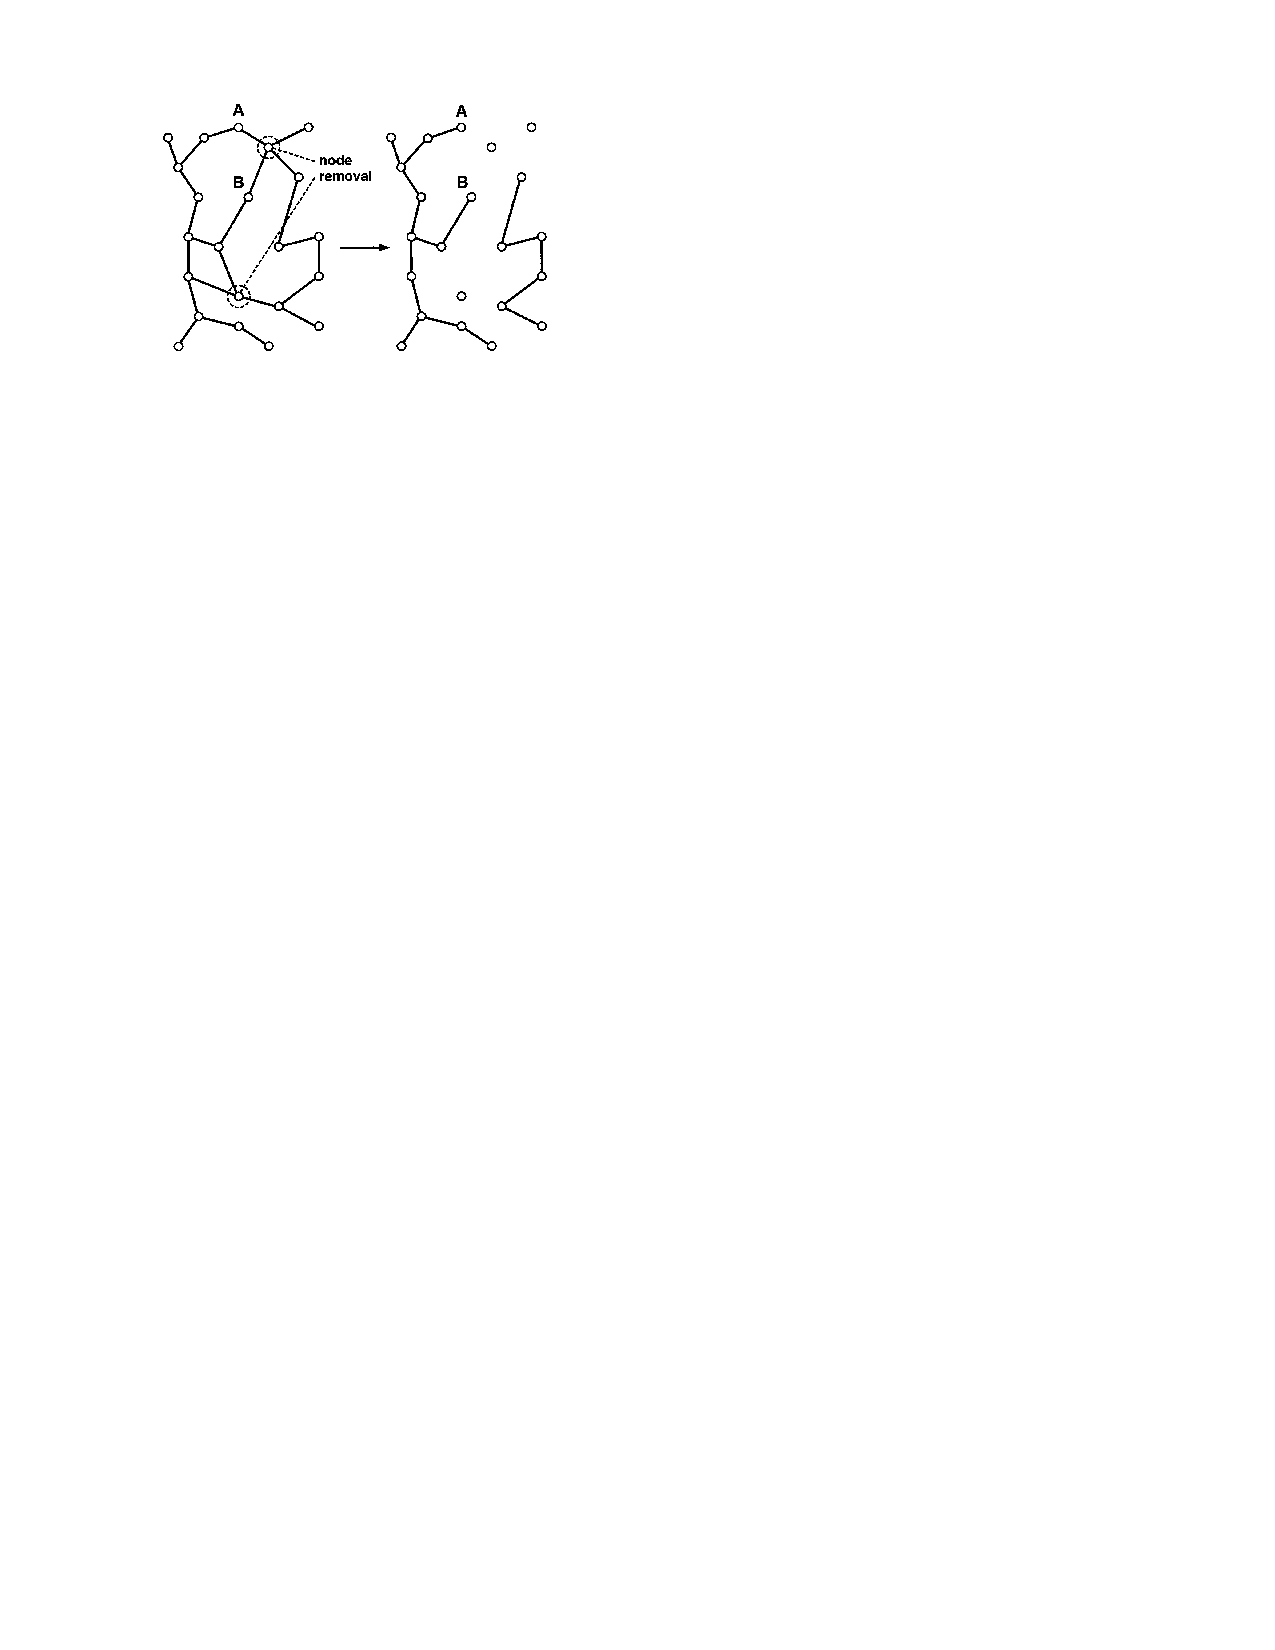
\includegraphics[width=\textwidth]{robustness1.pdf}
\end{figure}
\end{column}
\end{columns}

\end{frame}

\begin{frame}{Robustness}
	
\begin{columns}
\begin{column}{0.65\textwidth}
\begin{figure}
	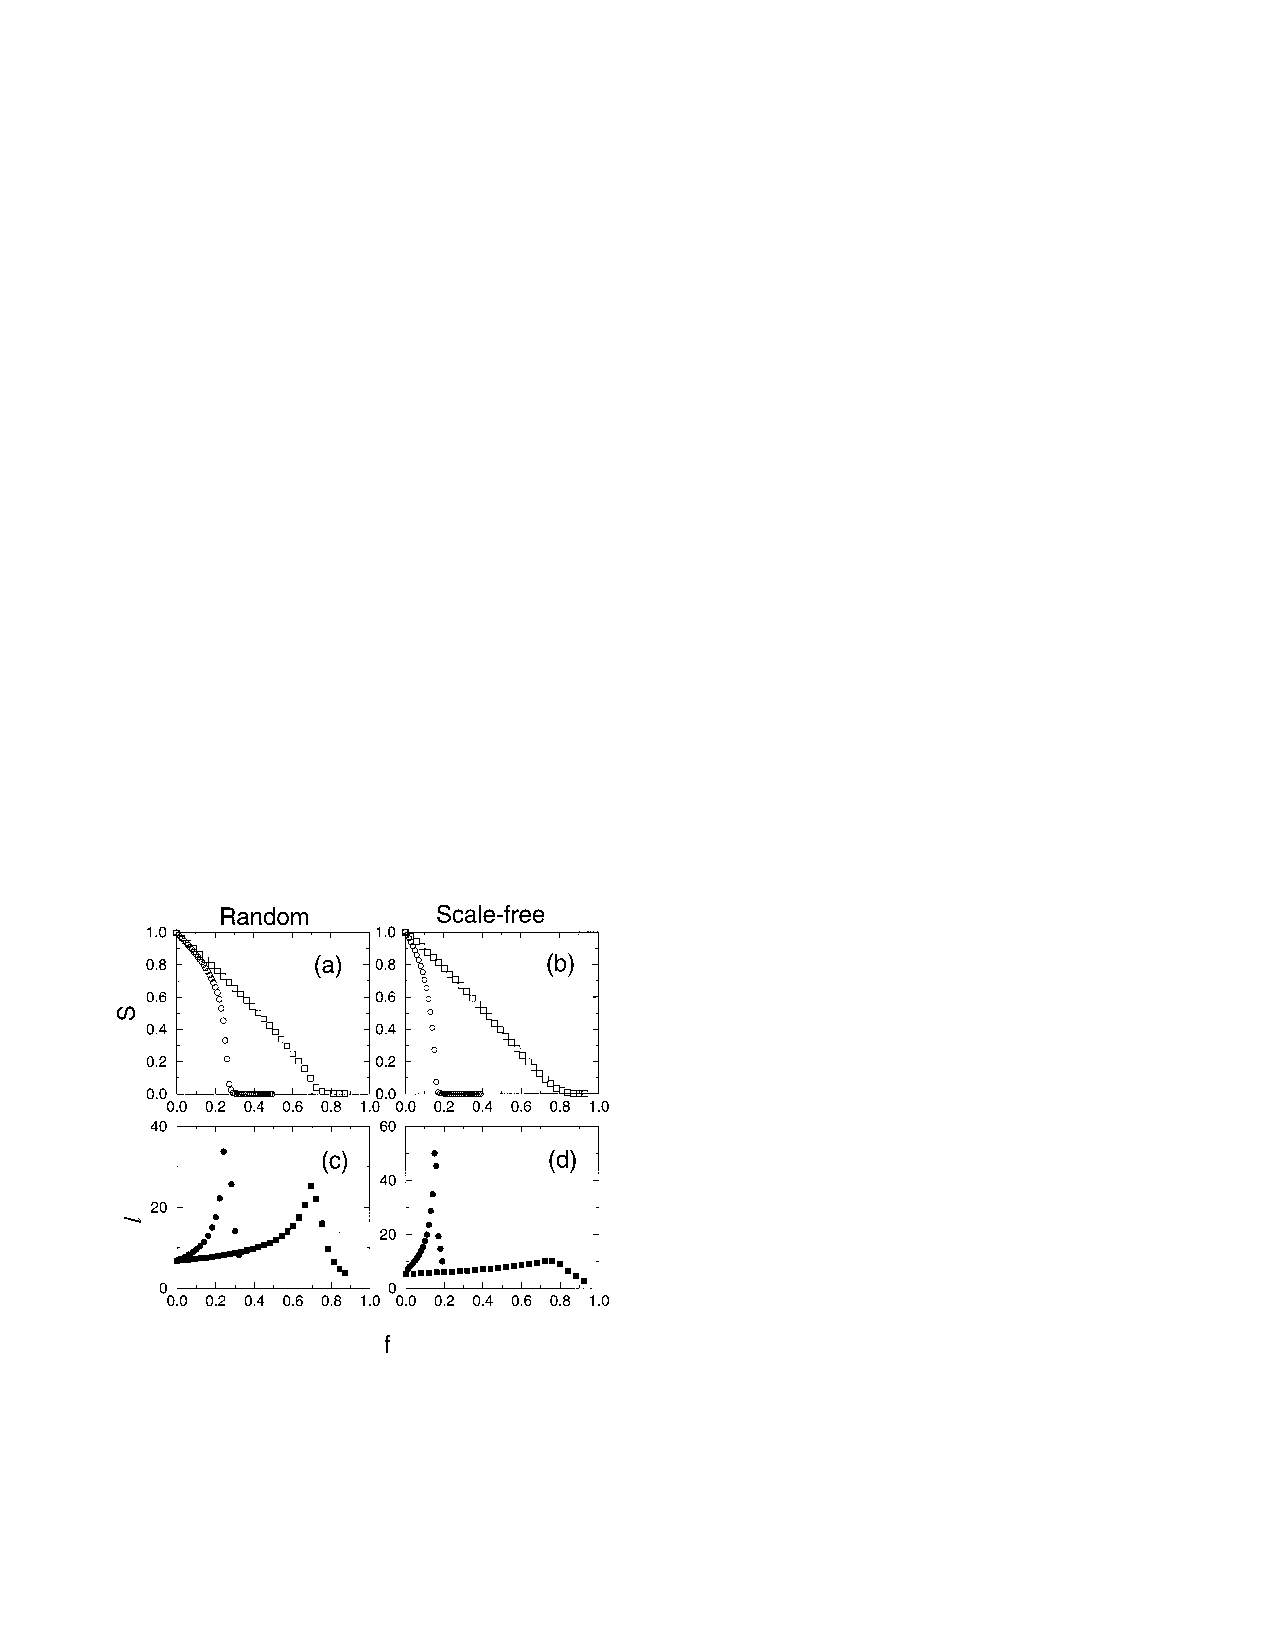
\includegraphics[width=\textwidth]{robustness2.pdf}
\end{figure}
\end{column}
\begin{column}{0.32\textwidth}
\BI
\item[(a,c)] random network, $N=10000$, $\langle k \rangle = 4$
\item[(b,d)] BA network, $N=10000$, $\langle k \rangle = 4$
\EI

\bigskip
\BI
\item[$\Box$] random removal\\
\item[$\circ$] preferential removal
\EI
\end{column}
\end{columns}



\note{
The relative size $S$ (a),(b) and average path length $l$ (c),(d) of the 
largest cluster in an initially connected network when a fraction $f$ of the nodes 
are removed. 
\BI
\item (a),(c) random network with $N=10000$ and $\langle k \rangle = 4$; 
\item (b),(d) scale-free network generated by the Barab\'{a}si-Albert model with $N=10000$ and $\langle k \rangle = 4$. 
\EI
Squares, random node removal; circles,  preferential removal of the most connected nodes.
}

\end{frame}

\begin{frame}{The story is not over...}

\BIL
\item $k$-core decomposition
\item Betweenness centrality
\item Closeness centrality
\item Eigenvector centrality
\item Cohesive subgroups
\item \ldots
\EIL


\end{frame}

\begin{frame}{Conclusions}
	
\structure{As computer scientists, what we can learn from complex networks?}
	
\BIL
\item Technological networks are resembling more and more to “real-life” networks
\item It opens a new topic of research: \alert{empirical computer science}
\item Measurement studies on:
  \BI
  \item BitTorrent,
  \item Internet, 
  \item WWW, \ldots
  \EI
\item Mathematical modeling is a useful tool, but it is not enough
\EIL	

\note{
 
\url{http://www.cs.jhu.edu/~nasmith/erm/}

Most of the computer science curriculum teaches you:
\BI
\item how to be a good engineer (e.g., computer programming, software engineering, and object-oriented
design), 
\item how to think about problems abstractly (e.g., algorithms, data
structures, theory of network communication, and automata theory)
\item how computing can be applied to solve various problems (e.g., vision, speech and
language processing, and transaction processing systems)
\item how computer systems work (e.g., operating systems). 
\EI

A different view is that computational objects (like computer programs) are
complex systems that sometimes need to be studied as one would study a
biological or physical system: by rolling up your sleeves and running
controlled experiments.

}
	
\end{frame}


%%%%%%%%%%%%%%%%%%%%%%%%%%%%%%%%%%%%%%%%%%%%%%%%%%%%%%%%%%%%%%%%%%%%%%%%

\begin{RMFrame}

\BI
\item \bibentry{complex-networks}
\EI

\end{RMFrame}

\end{document}